\chapter{相交树}
\label{chapter:geometric}
在这一章中,我们将按照图论里面的框架来介绍相交树的概念,并列出相交树的一些重要的性质。相交树的概念由刘春晖在他的文章~\inlinecite{Liu-multiplicity}中引入,主要是为了解决有限域上射影超平面上的重数计数问题。

在这一章中,我们总是预先取定了一个基域$k$。

\section{射影空间$\mathbb{P}^n$上的相交理论}
\label{subsection_intersection_theory}
% 首先我们来回忆一下重数的概念。令$X$为一个射影概型,$\xi\in X$为概型$X$的一个点。在式\eqref{local Hilbert-Samuel}中我们已经定义了点$\xi$在概型$X$中重数的概念,并将其记作$\mu_\xi(X)$。另外,如果$M$是概型$X$的一个整的闭子概型,并设其广点为$\eta_M$,我们把正整数$\mu_{\xi_M}(X)$定义为整闭子概型$M$在概型$X$中的重数,并将其简记作$\mu_M(X)$。

首先,我们需要回忆相交理论中一些有用的概念和性质,特别是射影空间$\mathbb{P}^n$上的相交理论。我们主要的参考文献是~\inlinecite{SerreLocAlg}以及~\inlinecite{Fulton}。相交理论是一个很广的课题,考虑到本文的需要以及为了简化起见,我们在本文中就不在最一般的框架下来介绍相交理论了。

设$Y$是域$k$上的正则的分离的概型,且在$k$上是有限型的。设$r \geqslant 2$是一个正整数,$X_1,\cdots, X_r$是$Y$的一组闭子概型,且它们都是维数纯的。有如下的 Cartesian 的图表
\begin{equation}
\begin{tikzcd}
X_1 \cap\cdots\cap X_r \arrow[r, hookrightarrow] \arrow[d] & X_1\times_k\cdots\times_k X_r \arrow[d] \\
Y\cong \Delta(Y) \arrow[r, hookrightarrow] & Y^{\times_k r}
\end{tikzcd}
\end{equation}
其中$\Delta: Y \to Y^{\times_k r}$为对角嵌入,$\bigcap\limits_{i=1}^r X_i =  X_1 \cap\cdots\cap X_r$为概型式交。记$\mathscr{I}$为作为$X_1\times_k\cdots\times_k X_r$闭子概型的$\bigcap\limits_{i=1}^r X_i$的理想层,也就是说
\begin{equation}
\mathscr{I} = \ker(\Delta^{\#}: \mathcal{O}_{X_1\times_k\cdots\times_k X_r} \to \Delta_{\ast} \mathcal{O}_{\bigcap\limits_{i=1}^r X_i}).
\end{equation}
设$M$为$\bigcap\limits_{i=1}^r X_i$的一个不可约分支。我们有下面的维数关系
\begin{equation}
\dim(M) \geqslant \dim(X_1) + \cdots + \dim(X_r) - (r-1)\dim(Y).
\end{equation}
如果上式的等号成立,那么称$X_1,\cdots, X_r$在$M$处正常相交,也称$M$是$\bigcap\limits_{i=1}^r X_i$的正常分支。如果$X_1,\cdots, X_r$在$\bigcap\limits_{i=1}^r X_i$的每一个不可约分支都是正常相交的,那么称$X_1,\cdots, X_r$是正常相交的。

设$M$是$\bigcap\limits_{i=1}^r X_i$的一个正常分支,$\Delta(M)$为$X_1\times_k\cdots\times_k X_r$整闭子概型。记$\Delta(M)$的广点为$\eta_{\Delta(M)}$,那么$X_1\times_k\cdots\times_k X_r$上的理想层$\mathscr{I}$在点$\eta_{\Delta(M)}$处的茎$\mathscr{I}_{\eta_{\Delta(M)}}$便是局部环$\mathcal{O}_{X_1\times_k\cdots\times_k X_r, \Delta(M)} = \mathcal{O}_{X_1\times_k\cdots\times_k X_r, \eta_{\Delta(M)}}$的一个理想,被称为对角理想。

\begin{definition} \label{multiplicity of proper component}
设$Y$是域$k$上有限型的的正则分离概型。设$r \geqslant 2$是一个正整数,$X_1,\cdots, X_r$是$Y$的一组闭子概型,且它们都是维数纯的。设$M$是$\bigcap\limits_{i=1}^r X_i$的一个正常分支,定义在$Y$中相交的$\bigcap\limits_{i=1}^r X_i$在$M$处的相交重数$i(M;X_1\intersect X_r;Y)$等于局部环$\mathcal{O}_{X_1\times_k\cdots\times_k X_r, \Delta(M)}$对于对角理想$\mathscr{I}_{\eta_{\Delta(M)}}$的重数,按照式\eqref{eq: multiplicity of a module}的写法,就是
\begin{equation} \label{eq: multiplicity of proper component}
i(M;X_1\intersect X_r;Y) = e_{\mathscr{I}_{\eta_{\Delta(M)}}
, \mathcal{O}_{X_1\times_k\cdots\times_k X_r, \Delta(M)}}.
\end{equation}
\end{definition}
如果基概型$Y$是很明确的,比如在本章考虑的问题中,基概型$Y$一直是射影空间$\mathbb{P}_k^n$,那么$i(M;X_1\intersect X_r;Y)$通常会被简写作$i(M;X_1\intersect X_r)$。为了方便书写,当$Y$的整闭子概型$N$不是$\bigcap\limits_{i=1}^r X_i$的子概形的时候,约定$i(N;X_1\intersect X_r;Y) = 0$。

如果$X_1,\cdots, X_r$是正常相交的,令$m = \dim(X_1) + \cdots + \dim(X_r) - (r-1)\dim(Y)$,那么相交积$X_1\intersect X_r$便是$\bigcap\limits_{i=1}^r X_i$上良定义的一个$m$-环元:
\begin{equation}
X_1\intersect X_r = \sum\limits_{M} i(M;X_1\intersect X_r;Y) {M}.
\end{equation}

我们将相交积$X_1\intersect X_r$的所有不可约分支组成的集合记为$\mathcal{C}(X_1\intersect X_r)$。若$X$为基概型$Y$的一个维数纯的闭子概型,那么$\mathcal{C}(X)$将表示$X$的所有不可约分支的集合。如果没有特别提到的话,集合$\mathcal{C}(X_1\intersect X_r)$以及$\mathcal{C}(X)$中的元素都被视为是基概型$Y$的整闭子概型。

\begin{proposition}[\inlinecite{Liu-multiplicity}, Th\'{e}or\`{e}me 3.3] \label{associativity of intersection}
设$Y$是域$k$上有限型的的正则的分离的概型。设$X_1,X_2,X_3$是$Y$的三个维数纯的闭子概型,且在$M\in \mathcal{C}(X_1\cdot X_2\cdot X_3)$处是正常相交的。那么
\begin{align}
i(M; X_1\cdot X_2\cdot X_3) & = \sum\limits_{P\in \mathcal{C}(X_1\cdot X_2)} i(M; P\cdot X_3)\cdot i(P; X_1\cdot X_2) \\
& = \sum\limits_{Q\in \mathcal{C}(X_2\cdot X_3)} i(M; Q\cdot X_1)\cdot i(Q; X_2\cdot X_3)
\end{align}
\end{proposition}
以上被称作是相交重数的结合性。这里,我们已经约定了,当$M$不是$P\cap X_3$或者$Q\cap X_1$的子概形的时候有$i(M; P\cdot X_3) = 0$或者$i(M; Q\cdot X_1) = 0$。注意以上命题与参考文献~\inlinecite{Fulton}的 Example 7.1.8 在叙述上的不同。此外,参考文献\inlinecite{Liu-multiplicity} Th\'{e}or\`{e}me 3.3 中提到的相交重数的交换性,在我们所考虑的这种最简单的框架下的相交,是显然的。但是,一般情况下的相交重数的交换性并不平凡,详见参考文献~\inlinecite{Fulton}的第七章。由此,也可以看出我们所定义的相交积的结合性:
\begin{equation}
X_1\cdot X_2\cdot X_3 = (X_1\cdot X_2)\cdot X_3 = X_1\cdot (X_2\cdot X_3),
\end{equation}
也就是说定义的相容性是很好的。


% \begin{proposition} \label{projection formula of intersection}
% 设$Y$是域$k$上有限型的的正则的分离的概型,$X$为$Y$的一个维数纯的闭子概型,$V,V'$为$Y$的有相同维数的两个子代数簇,$g: V' \to V$是满的本征态射。设$X$与$V$在$Z \in \mathcal{C}(X\cdot V)$处正常相交。若任一$M \in \mathcal{C}(g^{-1}(Z))$的维数都等于$\dim(V)+\dim(X)-\dim(Y)$,那么
% $$\deg(V'/V)\cdot i(Z, X\cdot V) = \sum\limits_{}$$
% \end{proposition}

% 对任意一个元素$M\in\mathcal C(X_1\intersect X_r)$,我们把相交积$X_1\intersect X_r$在$M$处的相交重数记作
% $$i(M;X_1\intersect X_r;Y).$$
% 关于相交重数的定义及其性质,可见参考文献~\inlinecite{Fulton}的第七章和第八章。

% 设$M\in\mathcal{C}(X_1\intersect X_r)$,$r\geqslant2$。一般地,我们有
% $$\dim(M)\geqslant\dim(X_1)+\cdots+\dim(X_r)-(r-1)\dim (Y),$$
% 见参考文献~\inlinecite{SerreLocAlg}第三章的 Proposition 17。如果上述不等式等号成立,并且相交非空的话,我们称$X_1,\cdots,X_r$在基概型$Y$中在$M$处正常相交。如果$X_1,\cdots,X_r$在他们相交积的所有不可约分支处都是正常相交的,那么我们称$X_1,\cdots,X_r$是正常相交的。

下面我们要介绍相交理论中非常重要的经典的定理,B\'ezout 定理。

我们设$\mathscr{L}$为一个丰沛的可逆$\mathcal{O}_Y$-模。如果$X$是基概型$Y$的闭子概型,我们将$X$的相对于$\mathscr{L}$的次数定义为
\begin{equation}
\deg_{\mathscr{L}}(X) := \deg(c_1(\mathscr{L})^{\dim(X)}\cap[X]).
\end{equation}
如果$\mathscr{L}$是泛丛$\mathcal{O}_Y(1)$,那么我们将把$X$关于泛丛$\mathcal{O}_Y(1)$的次数简记为$\deg(X)$,具体参见附录\ref{apdx: intersection theory}。或者更直观地,当$Y = \mathbb P^n_k$为$n$维射影空间,$X$由齐次理想$I(X)$定义时,有$X$次数的如下的定义。记$S(X) = k[T_0,\cdots,T_n] / I(X)$,为$X$的射影坐标环。$S(X)$是一个分次$k[T_0,\cdots,T_n]$-模,它的 Hilbert 多项式$P_{S(X)}$是一个次数等于$\dim(X)$的数值多项式,其最高次项系数的$(\dim(X))!$倍便是$X$的次数$\deg(X)$。
% \begin{equation}
% \varphi_{S(X)}()
% \end{equation}

B\'ezout 定理是一个利用我们以上定义的射影概型相对于泛丛的次数来描述作为基概型的射影空间$\mathbb P^n_k$上面的正常相交积的复杂程度的定理,把相交重数与概型的次数联系起来了,将会是证明有关相交树的一些结论的时候需要反复用到的定理。它的具体叙述如下

\begin{theorem}[B\'ezout 定理]
\label{bezout}
令$X_1,\cdots, X_r$为射影空间$\mathbb P^n_k$的一组纯维数的闭子概型。假设他们是正常相交的,那么有
\begin{equation} \label{eq: bezout}
\sum_{M\in\mathcal C(X_1\intersect X_r)}i(M;X_1\intersect X_r;\mathbb P^n_k)\deg(M)=\deg(X_1)\cdots\deg(X_r).
\end{equation}
\end{theorem}

关于 B\'ezout 定理更多的细节方面的东西,可以参考Fulton相交理论方面的的经典著作~\inlinecite{Fulton}的Proposition 8.4,或者该书第145页的等式(1)。

以下的命题将相交重数与闭子概型在母概型中的重数联系起来了,对于我们想要证明的结论来说,是一个非常重要的中间结果。

\begin{proposition} [\inlinecite{SamuelLocAlg}, 第六章, $n^\circ 1$, d, Proposition 1]
\label{relation of 2 kinds of multiplicities}
设基域$k$是一个完全域。设$X_1,\cdots, X_r$为射影空间$\mathbb P^n_k$的一组纯维数的闭子概型,$M\in \mathcal{C}(X_1\intersect X_r)$,那么有不等式
\begin{equation}
i(M;X_1\intersect X_r;\mathbb P^n_k) \geqslant \prod\limits_{i=1}^r \mu_M(X_i).
\end{equation}
\end{proposition}

\begin{remark}
Samuel 在\inlinecite{SamuelLocAlg}中使用了几何整这个条件但是未加强调,刘春晖在~\inlinecite{Liu-multiplicity}, Proposition 3.17 中把一般的情况补齐细节了。上面命题的证明可简述如下:由相交重数的定义\ref{multiplicity of proper component},相交重数$i(M;X_1\intersect X_r;\mathbb P^n_k)$等于局部环$\mathcal{O}_{X_1\times_k\cdots\times_k X_r, \Delta(M)}$的对于包含在其极大理想中的一个理想的重数,而$\mu_{\Delta(M)}(X_1\times_k\cdots\times_k X_r)$则是局部环$\mathcal{O}_{X_1\times_k\cdots\times_k X_r, \Delta(M)}$本身(关于其极大理想)的重数,因此由注释\ref{remarks on multiplicity of local rings}有
\begin{equation}
i(M;X_1\intersect X_r;\mathbb P^n_k) \geqslant \mu_{\Delta(M)}(X_1\times_k\cdots\times_k X_r).
\end{equation}
同样地,我们有
\begin{equation}
\mu_{\Delta(M)}(X_1\times_k\cdots\times_k X_r) \geqslant \mu_{M^{\times_k r}}(X_1\times_k\cdots\times_k X_r).
\end{equation}
其中,$M^{\times_k r}$表示$\underbrace{M\times_k\cdots\times_k M}_{\text{$r$重纤维积}}$。于是,想要得到上面命题的结论,只要证明
\begin{equation}
\mu_{M^{\times_k r}}(X_1\times_k\cdots\times_k X_r) = \prod\limits_{i=1}^r \mu_M(X_i)
\end{equation}
即可。上式是一个局部的结论,因此只要对$X_i$都是仿射的情况证明即可,而这可以由有关局部环张量积的重数的性质命题\ref{multiplicity of complete tensor}直接得出。
\end{remark}

\section{相交树的定义及其性质}
与上一小节一样,我们还是设$Y$是域$k$上的正则的分离的概型,$\mathscr{L}$为一个丰沛的可逆$\mathcal{O}_Y$-模。令$\delta \geqslant 1$为一个正整数,$\mathscr{T}$为一颗有根的树,其每条边有一个权重,每个顶点带了一个标签。称树$\mathscr{T}$为概型$Y$上级为$\delta$的相交树,如果$\mathscr{T}$满足下面的条件:
\begin{enumerate}
\item 树$\mathscr T$的每个顶点都是基概型$Y$的整闭子概型(一个整闭子概型可以作为树$\mathscr T$的顶点出现多次);
\item 树$\mathscr T$的每个顶点都被加上了一个标签,这个标签要么是空的,要么是基概型$Y$的纯维数的闭子概型;
\item 如果$X$是树$\mathscr T$的一个顶点,并且它不是叶节点,那么有下列条件要满足
	\begin{itemize}
	\item 顶点$X$的标签,记为$\widetilde{X}$,满足不等式$\deg_{\mathscr{L}}(\widetilde{X})\leqslant \delta$,还满足$X$和$\widetilde{X}$在基概型$Y$上正常相交;
	\item $X$的子节点都是$Y$上的相交积$X\cdot \widetilde{X}$的不可约分支;
	\item 对任意一个$X$的子节点$Z$ of $X$,连接这两个点的边$\ell$被赋予了一个权重$w_{\mathscr{T}}(\ell)$,等于相交积$X\cdot \widetilde{X}$在$Z$处的相交重数$i(Z;X\cdot \widetilde{X}; Y)$.
	\end{itemize}
\end{enumerate}

对于每个给定的相交树$\mathscr T$,称他的任意一个完全子树为$\mathscr T$的一个子相交树。每一个子相交树都是一个相交树。

相交树$\mathscr T$的每个顶点$X$也可以被赋予一个权重:顶点$X$与树$\mathscr T$的根节点有唯一的一条路径相连接,顶点$X$的权重就可以被定义为这条路径上所有的边的权重之积,记作$w_{\mathscr T}(X)$。特别地,如果$X$是相交树$\mathscr T$的根,那么我们约定$w_{\mathscr T}(X)=1$。

设$Z$是基概型$Y$的整闭子概型,我们也给它赋予一个在相交树$\mathscr{T}$中的权重。这个权重被定义作相交树$\mathscr{T}$中所有的作为基概型$Y$的整闭子概型等于$Z$的顶点的权重之和,记作$W_{\mathscr{T}}(Z)$。如果$Z$不作为顶点在相交树$\mathscr{T}$中出现,那么我们约定$W_{\mathscr{T}}(Z)=0$。需要说明的是,若$Z$是相交树$\mathscr{T}$的一个顶点,当我们写$W_{\mathscr{T}}(Z)$的时候,我们把$Z$视为基概型$Y$的一个整闭子概型,从而$W_{\mathscr{T}}(Z)$意思是,顶点$Z$作为整闭子概型的权重。也就是说我们需要把相交树$\mathscr{T}$中其他等于整闭子概型$Z$的顶点的权重也加进来。

下面,我们给出一些相交树的例子。

\begin{example}
\label{simple eg of intersection trees}
我们取仿射平面$\mathbb{A}_k^2 = \spec(k[X,Y])$为基概型,它在域$K$上显然是正则分离的。假设域$k$代数闭且其域特征$\operatorname{char}(k) \neq 2$。考虑其中的不可约的仿射平面曲线
\begin{equation}
C = \spec(k[X,Y] / (Y^2 + Y^4 + X^4 - X^3)),
\end{equation}
它的图像如下

\begin{figure}[H] % use float package if you want it here
\vspace{1cm}
\centering
\begin{psgraph}[Dy=10,Dx=10,arrows=->](0,0)(-0.4,-0.5)(1.3,0.5){9cm}{6cm}
\psplotImp[algebraic,linecolor=black,stepFactor=0.2](-0.4,-0.5)(1.3,0.5){y^2+y^4+x^4-x^3}
\end{psgraph}
\caption{平面曲线$C = \spec(k[X,Y] / (Y^2 + Y^4 + X^4 - X^3))$的图像}
\end{figure}

取$C$的标签为仿射直线
\begin{equation}
\widetilde{C} = \spec(k[X,Y] / (X)).
\end{equation}
于是$C\cap \widetilde{C}$为单点集$M = \{(0,0)\}$,是一个正常的相交,并且有
\begin{equation}
C\cdot \widetilde{C} = i(M; C \cdot \widetilde{C}; \mathbb{A}_k^2) \cdot M = 2 \cdot M.
\end{equation}
对于点$(0,0)$在$X$以及$\widetilde{X}$中的重数,有
\begin{equation}
\mu_{(0,0)}(C) = 2, ~~ \mu_{(0,0)}(\widetilde{C}) = 1.
\end{equation}
相关的相交树为
\begin{figure}[H]
\centering
\begin{tikzcd}
\dbox{$\widetilde{C} \cap $} C \phantom{he} 1 \arrow[d, "2"] \\
\phantom{hehe} \text{$M$} \phantom{he} 2 \\
\end{tikzcd}
\caption{以
平面曲线$C = \spec(k[X,Y] / (Y^2 + Y^4 + X^4 - X^3))$为根的一颗相交树}
\end{figure}
图中数字代表了相应的顶点或边的权重。除了退化为只有根节点的情况外,这是最简单的相交树。
% 在这个例子中,很容易验证前文的命题\ref{relation of 2 kinds of multiplicities}以及不久要阐述的关于相交树的主定理\ref{mult in the intersection tree}的正确性。
\end{example}

% \begin{example}
% 我们取射影平面$\mathbb{P}_k^2 = \proj(k[X,Y,Z])$为基概型,考虑其中的射影曲线
% $$X = \proj(k[X,Y,Z] / (Y^2 - Z^2)), ~~ \deg(X) = 2,$$
% 并取它的标签为射影直线
% $$\widetilde{X} = \proj(k[X,Y,Z] / (Z)), ~~ \deg(\widetilde{X}) = 1.$$
% 于是$X\cap \widetilde{X}$为单点集$[1:0:0]$,是一个正常的相交,并且有
% $$X\cdot \widetilde{X} = i([1:0:0]; X\cdot \widetilde{X}; \mathbb{P}_k^3) \cdot [1:0:0] = 2 \cdot [1:0:0].$$
% 这个简单的例子也可以验证B\'ezout 定理\ref{bezout}中等式\ref{eq: bezout}的正确性。对于点$[1:0:0]$在$X$以及$\widetilde{X}$中的重数,有
% $$\mu_{[1:0:0]}(X) = 2, ~~ \mu_{[1:0:0]}(\widetilde{X}) = 1.$$
% 相关的相交树为
% \begin{displaymath}
% \begin{tikzcd}
% \dbox{$\widetilde{X} \cap $} X \phantom{11} 1 \arrow[d, "2"] \\
% \text{$[1:0:0]$} \phantom{22} 2 \\
% \end{tikzcd}
% \end{displaymath}
% 图中数字代表了相应的顶点或边的权重。除了退化的情况外,这是最简单的相交树。在这个例子中,很容易验证前文的命题\ref{relation of 2 kinds of multiplicities}以及不久要阐述的关于相交树的主定理\ref{mult in the intersection tree}的正确性。
% \end{example}

本文需要解决的问题是射影的,因此接下来,我们举一个不那么平凡,稍微复杂一些的射影空间里面的相交树的例子。这个例子来自刘春晖的文章~\inlinecite{Liu-multiplicity}。

\begin{example}[\inlinecite{Liu-multiplicity}, Exemple 3.2]
\label{complicated eg of intersection trees}
取$4$维射影空间$\mathbb{P}_k^4 = \proj(k[T_0,T_1,T_2,T_3,T_4])$为基概型。考虑其中的两个超曲面:
\begin{equation}
X_1 = \proj(k[T_0,T_1,T_2,T_3,T_4] / (T_4)), ~~ \deg(X_1) = 1,
\end{equation}
以及
\begin{equation}
X_2 = \proj(k[T_0,T_1,T_2,T_3,T_4] / (T_3(T_0^2T_1-T_2^3+T_2^2T_1))), ~~ \deg(X_2) = 4.
\end{equation}
容易验证,$X_1$与$X_2$正常相交,$X_1\cap X_2$有以下的两个不可约分支
\begin{equation}
Y_1 = \proj(k[T_0,T_1,T_2,T_3,T_4] / (T_0^2T_1-T_2^3+T_2^2T_1, T_4)), ~~ \deg(Y_1) = 3,
\end{equation}
以及
\begin{equation}
Y_2 = \proj(k[T_0,T_1,T_2,T_3,T_4] / (T_3, T_4)), ~~ \deg(Y_1) = 1.
\end{equation}
相应的相交重数都等于$1$:
\begin{equation}
i(Y_1; X_1\cdot X_2; \mathbb{P}_k^4) = i(Y_2; X_1\cdot X_2; \mathbb{P}_k^4) = 1.
\end{equation}

取$Y_1$的标签为超曲面
\begin{equation}
\widetilde{Y}_1 = \proj(k[T_0,T_1,T_2,T_3,T_4] / (T_1T_3)), ~~ \deg(\widetilde{Y}_1) = 2;
\end{equation}
取$Y_2$的标签为
\begin{equation}
\widetilde{Y}_2 = \proj(k[T_0,T_1,T_2,T_3,T_4] / (T_0(T_0+T_1), T_2)), ~~ \deg(\widetilde{Y}_2) = 2.
\end{equation}
同样可以验证,$Y_1\cdot\widetilde{Y}_1$与$Y_2\cdot\widetilde{Y}_2$都是正常相交。

$\mathcal{C}(Y_1\cdot\widetilde{Y}_1)$有两个元素:
\begin{equation}
Y_{11} = \proj(k[T_0,T_1,T_2,T_3,T_4] / (T_1, T_2, T_4)), ~~ \deg(Y_{11}) = 1;
\end{equation}
以及
\begin{equation}
Y_{12} = \proj(k[T_0,T_1,T_2,T_3,T_4] / (T_0^2T_1 - T_2^3 + T_1T_2^2, T_3, T_4)), ~~ \deg(Y_{12}) = 3.
\end{equation}
对于它们的相交重数,有
\begin{gather}
i(Y_{11}, Y_1\cdot\widetilde{Y}_1; \mathbb{P}_k^4) = 3, \\
i(Y_{12}, Y_1\cdot\widetilde{Y}_1; \mathbb{P}_k^4) = 1.
\end{gather}
取$Y_{11}$的标签为超平面
\begin{equation}
\widetilde{Y}_{11} = \proj(k[T_0,T_1,T_2,T_3,T_4] / (T_0+T_3)),
\end{equation}
取$Y_{12}$的标签为超平面
\begin{equation}
\widetilde{Y}_{12} = \proj(k[T_0,T_1,T_2,T_3,T_4] / (T_2)).
\end{equation}
那么$\mathcal{C}(Y_{11}\cdot \widetilde{Y}_{11})$只有一个元素
\begin{equation}
Y_{111} = [1:0:0:-1:0],
\end{equation}
有相交重数$i(Y_{111}; Y_{11}\cdot \widetilde{Y}_{11}; \mathbb{P}_k^4) = 1$。而$\mathcal{C}(Y_{12}\cdot \widetilde{Y}_{12})$有两个元素
\begin{gather}
Y_{121} = [0:1:0:0:0], \\
Y_{122} = [1:0:0:0:0],
\end{gather}
分别有相交重数
\begin{gather}
i(Y_{121}; Y_{12}\cdot \widetilde{Y}_{12}; \mathbb{P}_k^4) = 2, \\
i(Y_{122}; Y_{12}\cdot \widetilde{Y}_{12}; \mathbb{P}_k^4) = 1.
\end{gather}

对于集合$\mathcal{C}(Y_2\cdot\widetilde{Y}_2)$,它有两个元素
\begin{gather}
Y_{21} = [0:1:0:0:0], \\
Y_{22} = [1:-1:0:0:0],
\end{gather}
其相交重数都等于$1$:
\begin{equation}
i(Y_{21}; Y_{2}\cdot \widetilde{Y}_{2}; \mathbb{P}_k^4) = i(Y_{22}; Y_{2}\cdot \widetilde{Y}_{2}; \mathbb{P}_k^4) = 1.
\end{equation}

注意到$0$维子概形,点$[0:1:0:0:0]$,作为图中的顶点出现了$2$次,分别为$Y_{21}$与$Y_{121}$。把相应的森林(由2颗相交树组成)画出来,就是
\begin{figure}[H]
\centering
\begin{tikzcd}
& Y_1 \arrow[dl, "3"'] \arrow[d, "1"] & Y_2 \arrow[dr, "1"] \arrow[d, "1"'] & \\
Y_{11} \arrow[d, "1"] & Y_{12} \arrow[dr, "1"] \arrow[d, "2"'] & Y_{21} & Y_{22} \\
Y_{111} & Y_{121} & Y_{122}
\end{tikzcd}
\caption{$4$维射影空间$\mathbb{P}_K^4$中的一颗相交树}
\end{figure}
上图的边的所带的数字是该边的权重,也就是相应的相交重数。图中还省略了顶点的标签。
\end{example}

\section{相交树上权重的估计}
为了进行有关权重的估计,我们首先需要引入下面的定理

\begin{theorem}[\inlinecite{Liu-multiplicity}, Th\'eor\`eme 3.1]
\label{mult in the intersection tree}
假设基域$k$是一个完全域。令$\{X_i\}_{i=1}^r$为作为基概型的射影空间$\mathbb P^n_k$的一族纯维数的闭子概型,并假设它们在基概型$\mathbb P^n_k$上正常相交。对相交积$X_1\intersect X_r$的每个不可约分支$C \in \mathcal C(X_1\intersect X_r)$,令$\mathscr T_C$为一个以$C$为根的相交树。我们在这一族相交树$\{\mathscr T_C\}_{C\in\mathcal C(X_1\intersect X_r)}$上,考虑满足如下条件的顶点$M$:

\vspace{2em}
\begin{minipage}[t]{\linewidth-3\parindent}
{\kaishu 任取这一族相交树$\{\mathscr T_C\}_{C\in\mathcal C(X_1\intersect X_r)}$中的一个顶点$Z$,如果$M$是$Z$的非平凡子概形,那么$M$就作为顶点$Z$的子孙而出现在$Z$所在的相交树中。}
\end{minipage}
\vspace{2em}

对于这样的顶点$M$,有如下的不等式成立:
\begin{equation}
\label{no auxillary scheme}
\sum_{C\in\mathcal C(X_1\intersect X_r)} W_{\mathscr T_C}(M)i(C;X_1\intersect X_r;\mathbb P^n_k)\geqslant \mu_{M}(X_1)\cdots\mu_{M}(X_r),
\end{equation}
% 其中$\mu_M(X_i)$为闭子概型$M$在$X_i$中的重数,定义可在本章开头找到。
\end{theorem}

% \begin{remark}
% 证明待写?

% \end{remark}

\begin{example}
接例\ref{complicated eg of intersection trees},记$M = [0:1:0:0:0]$,容易看出$M$满足定理\ref{mult in the intersection tree}中所提的条件。对于$M$在相交树$\mathscr T_{Y_1}$中的权重,有
\begin{equation}
W_{\mathscr T_{Y_1}}(M) = w_{\mathscr T_{Y_1}}(Y_{121}) = i(Y_{121}; Y_{12}\cdot \widetilde{Y}_{12}; \mathbb{P}_k^4) \cdot i(Y_{12}, Y_1\cdot\widetilde{Y}_1; \mathbb{P}_k^4) = 2\cdot1 = 2.
\end{equation}
而$M$在相交树$\mathscr T_{Y_2}$中的权重有
\begin{equation}
W_{\mathscr T_{Y_2}}(M) = w_{\mathscr T_{Y_2}}(Y_{21}) = i(Y_{21}, Y_2\cdot\widetilde{Y}_2; \mathbb{P}_k^4) = 1.
\end{equation}
于是
\begin{equation}
W_{\mathscr T_{Y_1}}(M) \cdot i(Y_1, X_1 \cdot X_2; \mathbb{P}_k^4) + W_{\mathscr T_{Y_2}}(M) \cdot i(Y_2, X_1 \cdot X_2; \mathbb{P}_k^4) = 2 \cdot 1 + 1 \cdot 1 = 3.
\end{equation}

另一方面,容易验证,$M$作为闭子概型,在$X_1,X_2$中的重数分别为:
\begin{equation}
\mu_M(X_1) = 1, ~~ \mu_M(X_2) = 3.
\end{equation}
于是我们有
\begin{align}
\mu_M(X_1) \cdot \mu_M(X_2) & = 3 \nonumber \\
\leqslant 3 = & W_{\mathscr T_{Y_1}}(M) \cdot i(Y_1, X_1 \cdot X_2; \mathbb{P}_k^4) + W_{\mathscr T_{Y_2}}(M) \cdot i(Y_2, X_1 \cdot X_2; \mathbb{P}_k^4),
\end{align}
% $$\mu_M(X_1) \cdot \mu_M(X_2) = 3 \leqslant 3 = W_{\mathscr T_{Y_1}}(M) \cdot i(Y_1, X_1 \cdot X_2; \mathbb{P}_k^4) + W_{\mathscr T_{Y_2}}(M) \cdot i(Y_2, X_1 \cdot X_2; \mathbb{P}_k^4),$$
符合定理\ref{mult in the intersection tree}的预测。
\end{example}

为了以后叙述以及证明的方便,我们需要在这里引进一些记号。在以下的定义中,我们保持在定理\ref{mult in the intersection tree}出现过的符号意义不变。

\begin{definition} \label{def of C_s}
令$t\in\mathbb{N}$为一个非负整数。我们把集合$\mathcal C_t$定义作所有的在相交树$\mathscr T_C$中深度为$t$的顶点构成的集合,其中相交树$\mathscr T_C$的下标$C$跑遍集合$\mathcal C(X_1\intersect X_r)$,即相交积$X_1\intersect X_r$的所有不可约分支组成的集合。

此外,我们还定义集合
\begin{equation}
\mathcal C_*=\bigcup\limits_{t\geqslant0}\mathcal C_t.
\end{equation}
\end{definition}

对每个非负整数$t$,我们还要定义另外一个重要的集合,作为集合$\mathcal C_t$的子集

\begin{definition} \label{def of Z_s}
我们定义集合$\mathcal Z_t$为集合$\mathcal C_t$中满足如下条件的元素$M$构成的子集合: 任取这一族相交树$\{\mathscr T_C\}_{C\in\mathcal C(X_1\intersect X_r)}$中的一个顶点$Z$,如果$M$是$Z$的非平凡子概形,那么$M$就作为顶点$Z$的子孙而出现在$Z$所在的相交树中。

此外,我们还定义集合
\begin{equation}
\mathcal Z_*=\bigcup\limits_{t\geqslant0}\mathcal Z_t.
\end{equation}
\end{definition}

由定义,有$\mathcal Z_0=\mathcal C_0=\mathcal C(X_1\intersect X_r)$。注意到$\mathcal Z_*$正是在定理\ref{mult in the intersection tree}中满足不等式\eqref{no auxillary scheme}的那些顶点。

为了更好地理解集合$\mathcal Z_*$,我们来举一个例子。
\begin{example}
考虑如下的一族相交树(深度大于$1$的点未画出)。
\begin{figure}[H]
\centering
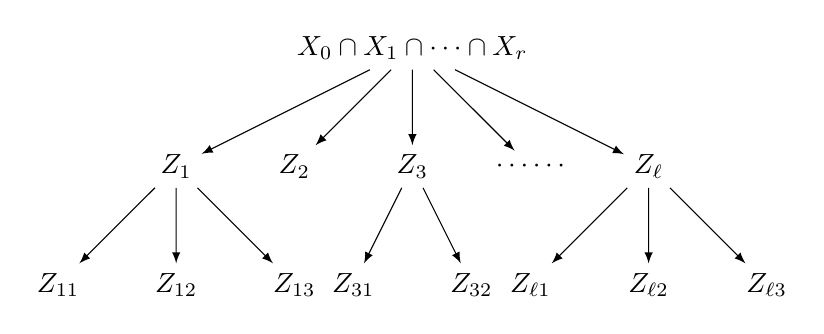
\begin{tikzpicture}[edge from parent/.style={draw,-latex}]
% [edge from parent/.style={draw, ->, thick}, level/.style={sibling distance = 30mm/#1, yshift=5cm}]
% \tikzstyle{level 2}=[sibling distance=15mm]
% \tikzstyle{level 3}=[sibling distance=5mm]
\node {$X_0\cap X_1\cap\cdots\cap X_r$} % root
child { node {$Z_1$}
child { node {$Z_{11}$} }
child { node {\dbox{$Z_{12}$}} }
child { node {$Z_{13}$} }
}
child { node {$Z_2$}
}
child { node {$Z_3$}
child { node {$\boxed{Z_{31}}$} }
child { node {$Z_{32}$} }
}
child { node {$\cdots\cdots$}
}
child { node {$\boxed{Z_{\ell}}$}
child { node {$Z_{\ell1}$} }
child { node {$Z_{\ell2}$} }
child { node {\dbox{$Z_{\ell3}$}} }
};
\end{tikzpicture}
\caption{以$X_0\cap X_1\cap\cdots\cap X_r$的不可约分支为相交树根构成的森林}
\end{figure}
假设虚线框中的顶点$Z_{12}$对应的$\mathbb{P}_k^n$的闭子概型同时是$Z_1, Z_{\ell}\in \mathcal{C}(X_1\intersect X_r)$的子概形,而且这个子概形作为$Z_{\ell}$的子节点,是另一个虚线框中的$Z_{\ell3}$,而出现在相交树中。于是,相关的顶点$Z_1, Z_{\ell}$便是集合$\mathcal Z_*$,确切的说是集合$\mathcal Z_1$,中的元素。

再假设实线框中的顶点$Z_{31}$所对应的$\mathbb{P}_k^n$的闭子概型同时是$Z_3, Z_{\ell}\in \mathcal{C}(X_1\intersect X_r)$的子概形,但是这个子概形并未作为$Z_{\ell}$的子节点而出现,因此它便不落在集合$\mathcal Z_*$中。
\end{example}

\begin{remark}
要注意的是,在上面的例子中,$Z_1,\cdots,Z_{\ell}$才是每棵相交树的根,深度为$0$。事实上,如果我们把相交树族$\{\mathscr T_C\}_{C\in\mathcal C(X_1\intersect X_r)}$视作一个森林$\mathcal{F}_{C(X_1\intersect X_r)}$,把$X_0\cap X_1\cap\cdots\cap X_r$当成一个顶点,与森林$\mathcal{F}_{C(X_1\intersect X_r)}$中所有根相连,从而把所有相交树连接成一棵树的话,再扩展相关顶点以及边的权重的定义,某些式子能得到简化,例如不等式\eqref{no auxillary scheme}左边不再需要求和,变成只有一项,但是抽象的相交树的定义相关的叙述会变得更繁琐和不统一。于是,本文还是尊重最初提出相交树的~\inlinecite{Liu-multiplicity}中的定义。
\end{remark}

\begin{remark}
我们特别地将集合$\mathcal Z_*$从集合$\mathcal C_*$中拿出来考虑,是因为被丢弃的那些顶点对应的闭子概型中点的重数已经在别处得到了计算与控制,例如上例中的$Z_{31}$与$Z_{\ell}$,因此我们不重复计算。
\end{remark}

\begin{definition}
令$t$为一个非负整数。我们将集合$\mathcal C_t$,$\mathcal Z_t$,$\mathcal C_*$以及$\mathcal Z_*$中的元素(相交树的顶点)所对应的标签构成的集合分别记为$\mathcal C'_t$,$\mathcal Z'_t$,$\mathcal C'_*$以及$\mathcal Z'_*$。
\end{definition}

下面我们要给出关于我们以上定义的集合的一个重要的性质。这个性质是定理\ref{mult in the intersection tree}的推论,将会直接用于我们所考虑的重数计数问题的证明。

\begin{proposition}[\inlinecite{Liu-multiplicity}, Proposition 4.6] \label{grassmanne}
我们保持定理\ref{mult in the intersection tree}中的记号与条件不变,并假设由相交树顶点标签组成的集合$\mathcal C'_*$的每个元素(对应的基概型的整闭子概型)维数都相同,那么对每个$0\leqslant t \leqslant s$有不等式
\begin{equation} \label{relation of multiplicity and degree}
\sum_{Z\in \mathcal Z_t} \left(\prod_{i=1}^r\mu_Z(X_i)\right)\deg(Z) \leqslant \prod_{i=1}^r\deg(X_i)\prod_{j=0}^{t-1}\max_{\widetilde{M}\in \mathcal C'_j}\{\deg(\widetilde{M})\}.
\end{equation}
特别地,在上式中,如果$t=0$,我们约定$\prod\limits_{j=0}^{t-1} \max\limits_{\widetilde{M}\in \mathcal C'_j} \{\deg(\widetilde{M})\} = 1$。
\end{proposition}

\begin{proof}
由定理\ref{mult in the intersection tree},对集合$\mathcal{Z}_*$中所有的顶点$Z$有
\begin{equation}
\sum_{C\in\mathcal C(X_1\intersect X_r)} W_{\mathscr T_C}(Z)i(C;X_1\intersect X_r;\mathbb P^n_k) \geqslant \prod_{i=1}^r\mu_Z(X_i),
\end{equation}
又注意到$\mathcal{Z}_t$是$\mathcal{C}_t$子集,因此
\begin{multline}
\sum\limits_{Z\in \mathcal{Z}_t} \left( \sum_{C\in\mathcal C(X_1\intersect X_r)} W_{\mathscr T_C}(Z)i(C;X_1\intersect X_r;\mathbb P^n_k) \right)\deg(Z) \\
\leqslant \sum\limits_{Z\in \mathcal{C}_t} \left( \sum_{C\in\mathcal C(X_1\intersect X_r)} W_{\mathscr T_C}(Z)i(C;X_1\intersect X_r;\mathbb P^n_k) \right)\deg(Z)
\end{multline}
恒成立。于是想要证明不等式\eqref{relation of multiplicity and degree},我们只要证明下式即可:
\begin{align}
I_t := & \sum\limits_{Z\in \mathcal{C}_t} \left( \sum_{C\in\mathcal C(X_1\intersect X_r)} W_{\mathscr T_C}(Z)i(C;X_1\intersect X_r;\mathbb P^n_k) \right)\deg(Z) \\
& \leqslant \prod_{i=1}^r\deg(X_i)\prod_{j=0}^{t-1} \max_{\widetilde{M}\in \mathcal C'_j} \{\deg(\widetilde{M})\} =: J_t.
\end{align}

我们对$t$进行归纳证明。

当$t=0$时,$\mathcal{C}_0 = \mathcal C(X_1\intersect X_r)$,因此
\begin{equation}
W_{\mathscr T_C}(Z) = \begin{cases}
1 & \text{ 如果$Z = C$;} \\
0 & \text{ 如果$Z \neq C$.}
\end{cases}
\end{equation}
由B\'ezout 定理(定理\ref{bezout})有
\begin{equation}
I_0 = \sum_{C\in \mathcal C(X_1\intersect X_r)} i(M;X_1\intersect X_r;\mathbb P^n_k) \deg(C) = \deg(X_1)\cdots\deg(X_r) = J_0.
\end{equation}

设$t\geqslant 1$,且命题在$t-1$时成立。那么对$t$有归纳假设有
\begin{align}
J_t & = \max_{\widetilde{M} \in \mathcal C'_{t-1}} \{\deg(\widetilde{M})\} \cdot J_{t-1} \geqslant \max_{\widetilde{M}\in \mathcal C'_{t-1}} \{\deg(\widetilde{M})\} \cdot I_{t-1} \\
& = \max_{\widetilde{M}\in \mathcal C'_{t-1}} \{\deg(\widetilde{M})\} \cdot \left( \sum\limits_{Z\in \mathcal{C}_{t-1}} \left( \sum_{C\in\mathcal C(X_1\intersect X_r)} W_{\mathscr T_C}(Z)i(C;X_1\intersect X_r;\mathbb P^n_k) \right)\deg(Z) \right) \\
& \geqslant \sum\limits_{Z\in \mathcal{C}_{t-1}} \left( \sum_{C\in\mathcal C(X_1\intersect X_r)} W_{\mathscr T_C}(Z)i(C;X_1\intersect X_r;\mathbb P^n_k) \right) \deg(Z) \deg(\widetilde{Z}) \\
& = \sum\limits_{Z\in \mathcal{C}_{t-1}} \left( \sum_{C\in\mathcal C(X_1\intersect X_r)} W_{\mathscr T_C}(Z)i(C;X_1\intersect X_r;\mathbb P^n_k) \right) \cdot \sum\limits_{Z'\in \mathcal{C}(Z\cdot \widetilde{Z})} i(Z'; Z\cdot \widetilde{Z}; \mathbb P^n_k) \deg(Z') \\
& = \sum\limits_{Z'\in \mathcal{C}_{t}} \left( \sum_{C\in\mathcal C(X_1\intersect X_r)} W_{\mathscr T_C}(Z)i(C;X_1\intersect X_r;\mathbb P^n_k) \right) \deg(Z') \\
& = I_t.
\end{align}
在上式中,第三行我们用$\widetilde{Z}$表示顶点$Z$对应的标签;第四行我们再一次用到了B\'ezout 定理(定理\ref{bezout});第五行则用到了相交重数的结合性(命题\ref{associativity of intersection})。于是命题得证。
\end{proof}
